\documentclass[10pt,twocolumn,letterpaper]{article}

\usepackage{cvpr}
\usepackage{times}
\usepackage{epsfig}
\usepackage{graphicx}
\usepackage{amsmath}
\usepackage{gensymb}
\usepackage{amssymb}
\usepackage{float}
\usepackage{mathtools}
\usepackage{subcaption} 
\usepackage{booktabs}
\DeclarePairedDelimiter{\ceil}{\lceil}{\rceil}

% Include other packages here, before hyperref.

% If you comment hyperref and then uncomment it, you should delete
% egpaper.aux before re-running latex.  (Or just hit 'q' on the first latex
% run, let it finish, and you should be clear).
\usepackage[breaklinks=true,bookmarks=false]{hyperref}

\cvprfinalcopy % *** Uncomment this line for the final submission

\def\cvprPaperID{****} % *** Enter the CVPR Paper ID here
\def\httilde{\mbox{\tt\raisebox{-.5ex}{\symbol{126}}}}

% Pages are numbered in submission mode, and unnumbered in camera-ready
% \ifcvprfinal\pagestyle{empty}\fi
\begin{document}

%%%%%%%%% TITLE
\title{
    DeepCube: Transcribing Rubik's Cube Moves with Action Recognition
}

\author{Junshen Kevin Chen\\
Stanford University\\
{\tt\small jkc1@stanford.edu}
\and
Wanze Xie\\
Stanford University\\
{\tt\small wanzexie@stanford.edu}
\and
Zhouheng Sun\\
Stanford University\\
{\tt\small sunz@stanford.edu}
}

\maketitle

\begin{abstract}

% this is too much detail for abstract

Transcribing Rubik's Cube moves from videos is a frequent work in speedcubing communities and often done manually. Inspired by the success of action recognition in computer vision, we hope to automate this process using deep learning techniques. In this work, we introduce DeepCube, an egocentric video dataset of turning Rubik's cube under a controlled environment. DeepCube contains 20K trimmed video clips and 50 temporally localized untrimmed videos annotated with 22 Rubik's cube move classes. We demonstrate the performance of two tasks on DeepCube, achieveing 83.5\% Top-1 accuracy and 78.4\% mAP for video classification, and Edit Distance Per Frame (EDPF) of 0.0037 for action sequence recognition. In particular, we propose a novel model to achieve sequence recognition and introduced a new framework for evaluation. Our work shows the promise of enabling automatic transcribing for speedcubing competitions as well as contributes to the study of sequential action recognition for atomic visual activities.

\end{abstract}


\section{Introduction}
Speedcubing, namely solving a Rubik's Cube as fast as possible, has been a long standing sport since its invention. With the popularity of the sport, there is a constant interest for players and learners to watch videos of cube solves in competitions, transcribe the moves manually into text, and submit the solution sequence to speedcubing communities such as CubeSolves \cite{CubeSolves}. With recent advance in video understanding and action recognition, we hypothesize that the process of manually transcribing Rubik's Cube moves can be automated using vision-based deep learning approaches. We are motivated that our study can further facilitate the sport of speedcubing.

On the other hand, while action recognition has been popular and successful in detecting various human activities \cite{charades, ava, kinetics, finegym, hvu}, studies on the fine-grained atomic actions has been relatively scarce, mainly due to the lack of well-defined atomic activities. This motivates the problem of action recognition for Rubik's Cube operations, a subtle and atomic activity that is challenging to detect. Moreover, the Rubik's moves are often short and sequential, which ties to another less explored topic, referred as action sequence detection \cite{ng2019human, action_sequence_movie}. As such, we also aim this study to push forward the frontier of vision-based fine-grained atomic action recognition and action sequence detection.

\begin{figure}[]
    \centering
    \includegraphics[scale=0.35]{explain.png}
    \caption{The DeepCube dataset include the temporal labels and action labels for cube moves in the video. This figure shows two example movements, with transcription '$\text{D}'$, $\text{U}'$'.}
    \label{fig:recording_setup}
    \vspace{-2mm}
\end{figure}

To tackle this problem, we introduce DeepCube, an egocentric video dataset of a person turning a Rubik's Cube under a controlled environment. Our dataset is collected by us in well-lit environments with static monotonic background. It contains 20K trimmed video clips and 50 temporally localized untrimmed videos totalling over 150 minutes of continuous play. Each performed move is annotated by one of the 22 possible cube move classes. 

Then, we formulate the problem in two ways: (1) a \textbf{multi-class video classification task}, where we segment the videos into individual moves, and design models to classify the single move performed in each segment, and (2) an \textbf{action sequence stream recognition task}, where we use an arbitrary length video as input, and design model to output the arbitrary number of moves performed in the segment, in the correct order.

We first demonstrate that recognizing Rubik's Cube operation is viable through vision-based deep learning approaches by showing that multi-class classification for trimmed video clips can achieve  78.4\% mAP, with 83.5\% Top-1 accuracy, 96.8\% Top-5 accuracy using R3D \cite{r3d}. 

For the action sequence recognition task, we experiment with a 3D convolutional model, an optimized LRCN, and a LRCN augmented by 3D temporal features to achieve the best result. We propose edit distance per frame (EDPF), a new metric to evaluate sequence recognition tasks, and show that our best-performing 3D-LRCN model achieves a test EDPF of ~0.0037, or about one mistake per 9 seconds of video, making it viable for in practical applications.


\section{Related Work}

While there exists a few research that explores the marriage between rubik's cube and deep learning \cite{cube_robotics, cube_rl}, they are related to constructing solution based on cube's current state with reinforcement learning \cite{cube_rl} and robotics \cite{cube_robotics}. Our work differs in that we want to detect cube's moves rather than constructing solution for it. Therefore our inspirations primarily draw from action recognition in videos. 
\vspace{-2mm}

\paragraph{Action Recognition Datasets.} Previously, most action recognition datasets focus on video classification, such as hollywood2 \cite{hollywood2}, UCF101 \cite{ucf101}, and YouTube-8M \cite{youtube8m}. These datasets are suited for tasks that directly maps the whole video clip to an action class. More recently, more works shift toward to temporal localization for activities. The datasets like Charades \cite{charades} and ActivityNet \cite{activitynet} contains long videos 
with multiple actions occurring at different time period. AVA \cite{ava} steps further and introduces spatio-temporal localization of actions and highlights the concept of atomic actions. Although most of the aforementioned datasets are allocentric, there exist a few egocentric video datasets like Something-something \cite {sthsth} and EPIC-Kitchens \cite{epic_kitchen}, but none focuses on atomic visual activities. This is where our work fits in - an egocentric video datasets for temporal atomic action localization in a specific task.

\paragraph{Action Classification and Detection.} Although there are some non deep learning-based attempts \cite{sadek2012fast, stochastic} for recognizing human activities, a vast majority of action models with impressive results come from architecture that leverages deep learning techniques. One popular structure involves using CNN to extract visual features and feed into an RNN module for sequence learning, which allows variable-length visual input and class label output, known as LRCN \cite{lrcn}. Some modern state-of-the-art models \cite{ava, better_ava} often combines a "backbone" 3D CNN, such as I3D \cite{i3d} and R3D \cite{r3d}, with a region detector using Faster R-CNN \cite{faster_rcnn}, followed by a classifier for video classification, or by a proposal network \cite{ss-tad, g-tad} for action detection. 

For action sequence recognition, there are some work focused on learning order of activities to generate natural language description \cite{ng2019human} or retrieve action sequence in movies \cite{action_sequence_movie}, but they only focused on the sequence of 3 or 4 actions. However, in our Rubik's Cube setting, a couple seconds in the clip can incorporate 10 to 30 different actions due to the fast operations when solving the cube. Therefore, we highlight one of our tasks as action sequence stream detection, and we study the approach to recognize a stream of sequence of atomic actions in video clips of any length. 


\section{Data}

% \textit{Clearly describe the dataset and any pre-processing steps. If you are collecting your own dataset or your project requires significant effort in data preprocessing, describe your work on the dataset collection / pre-processing pipeline clearly in a standalone subsection.}

We collect our own original dataset. We first present the format of our data, and then describe the collection process.
\vspace{-5mm}

\paragraph{Format and Definitions.} 
The dataset is a collection of annotated video clips of a human solver playing a Rubik's Cube. We consider a cube move or rotation (as explained below) as an atomic action. One action will be marked by one label attached to one frame that correspond to the \textbf{end} of that action. For frames with no actions, a zero label is attached. As such, every frame of the video is annotated with one label. Labels fall into the following categories, with a total of 22 classes:
\begin{enumerate}
    \itemsep 0em
    \item \textit{No action}, denoted by $\emptyset$.
    \item \textit{Layer moves}. These describe a 90-degree turn of one of the six outer layers of the cube, clockwise or counterclockwise, denoted as U,D,F,B,L,R and U',D',F',B',L',R', respectively. Their 180 degree counterparts are modeled as consecutive repeats of 90-degree moves, and do not require labels on their own.
    \item \textit{Cube rotations}. These describe a whole-cube rotation. We assume rotations only happen around the x, y or z axis, and could be 90$\degree$ clockwise (x, y, z), 90$\degree$ counterclockwise (x', y', z'), or 180$\degree$ with no specific direction of rotation (x2, y2, z2). 
\end{enumerate}

\paragraph{Collection Pipeline.}
We record moves using a camera facing the cube from the general direction of the solver, such that only the up and front faces are visible most of the time. The hands of the solver must be fully visible, against a uniform dark background. The solver proceeds to do regular scrambles and solves at medium speed, so that motion blur is minimized. 

% \begin{figure}[]
%     \centering
%     \includegraphics[scale=0.15]{recording_setup.png}
%     \caption{Sample frames from DeepCube dataset. The right image is performing a move labeled as ‘L’.}
%     \label{fig:recording_setup}
%     \vspace{-2mm}
% \end{figure}

To obtain the timestamp of each turn, we use a commercial bluetooth-connected Rubik's Cube that emits signals for cube moves and orientations, sending a packet at \char`\~100ms intervals as soon as it detects an action is complete. We write a program that captures the signal while we are recording, and processes the signals to (timestamp, label) pairs. After recording finishes, we play the video and the annotation side by side, and manually align annotation timestamps with the video frames with a global offset, to obtain (frame, label) pairs. Again, each label is aligned with the frame at which the corresponding action is considered finished by human viewers. Finally, frame without annotations are assigned the zero-label.

\paragraph{Dataset Statistics.}
In total there are more than 150 minutes of video footage recorded at 30 fps, which contains 20K trimmed video clips and 50 temporally localized untrimmed video. Each performed move is annotated by one of the 22 possible cube move classes. 

\paragraph{Temporal Localization.} For the trimmed video classification task, we require temporal localization for the action labels so as to segment video clips based on the start and end time of the action. Since we have in over 20K instances of moves in the entire dataset, so we adopt an efficient approach to automatically generate most of the start and end labels for the actions. 

In our aligned annotation file, the "finish" time of each cube moves has already been included, so we infer the start time of the cube actions based on the assumption that (1) the majority of the actions are continuous and (2) all actions are completed within at most 2 seconds. As a result, we label the next frame the previous action's end as the start frame of the next action. We empirically constrain the action duration within 3 to 50 frames, labeling the intervals larger than 50 frames as no actions. However, during the training time, we also have the flexibility to set the minimum accepted frame number to further exclude extremely short video clips to counteract the noise label generated by the smart cube sensor.

\section{Methods}
As an overview, in 4.1 we describe the model for the multi-class video classification task, in which our goal is to predict the action label given a trimmed video clip that is expected to contain only one action. Then in 4.2 to 4.4 we describe 3 different approaches for the action sequence stream recognition task, where the goal is to predict a variable-length sequence of actions showed in a given fixed-length video clip. Lastly, in 4.5 and 4.6 we describe the techniques we have adopted during the training of both tasks.

\subsection{3D Residual Convolutional Network}
To demonstrate the utility of DeepCube on the video classification task, we utilize ResNet \cite{resnet}, and specifically ResNet with 3D Convolution (R3D) \cite{r3d} to perform the classification task. The model takes in preprocessed video segment based on the temporal labels, and predict one action label out of the 22 possible cube move classes.

Based on \cite{resnet} and \cite{r3d}, we create R3D networks that support different model depth, and we particularly focus on 10 layer, 50 layer and 101 layer networks. The model takes in a video clip of shape $(C, L, H, W)$ where in our case $C=3$, $H=68$ and $W=90$. $L$ stands for the clip length and depends on the minimum accepted frame. The model performs a 3D convolution with 3x7x7 kernel that preserves resolution in the first layer and then expand to 4 types of layers with hidden size 64, 128, 256, and 512, followed by 3D adaptive average pooling and an FC layer to produce 22 class scores. When building layers, we followed the original design \cite{resnet} and used basic block for shallower networks and bottleneck unit for deeper networks.

As described in 3.3, we select the "minimum accepted frames", or clip length $L$, so that videos with frames fewer than $L$ are excluded, since extremely short clips are likely to be sensor noises rather than valid moves. With larger $L$, the model would have access to more information for a particular action. However, a larger $L$ also leads to fewer training samples, so we take $L$ as one of the hyperparameters for our models. For video clips that have length larger than $L$, we subsample frames from the video to match the clip length.

In terms of training, we use multi-class cross entropy loss and evaluate using Top-K accuracy and Mean Average Precision (mAP), which will be discussed further in 5.1. We also implemented a few data augmentation techniques for this task which are discussed in section 4.6. 

\subsection{3D Convolutional Sequence Recognizer}

\begin{figure}[]
    \centering
    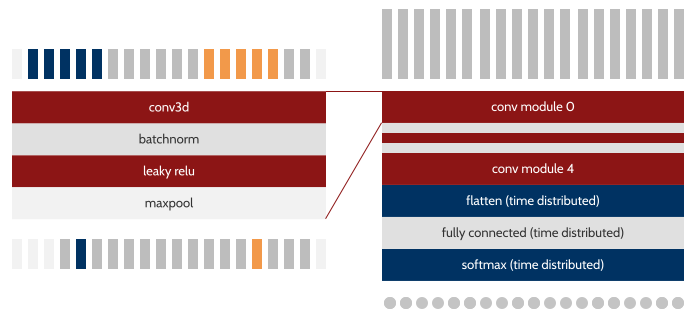
\includegraphics[scale=0.33]{3d-conv-clf.png}
    \caption{Feature extractors, space-wise dimension not depicted for frames, highlighted frames on top convolves to same-colored frame at bottom. Left: 3D convolutional feature extractor; Right: 2D convolutional feature extractor}
    \label{fig:3dconv}
\end{figure}



Intuitively, since we annotate each move in the video to be its movement label at its completion, and moves are entirely independent among one another, we may build a convolutional model that accepts an \textbf{input} of sequence of frames of images and produces \textbf{output} of a sequence of action class (including the no-movement class). Input sequences are of arbitrary length, and the convolution kernels acts as sliding window over the time axis as well as the space axes. 

\paragraph{3D Convolutional Feature Extractor.}

Figure \ref{fig:3dconv} describes a 3D convolutional feature extractor, consisting of a 3D convolutional layer, batch normalization, leaky ReLU activation, and max-pooling over the space dimensions. At each time step $t$, output is a feature matrix of size $(outChannel, outHeight, outWidth)$, which is produced by the convolving with input features in the time range of $(t-TimewiseKernelSize+2, t+1)$, since we annotate the movement near its finishing frame, so we value previous frame more than the latter ones, to better replicate an on-line scenario. The input frames are zero-padded time-wise to maintain output length.

\paragraph{Time-distributed Feed-forward Network.}

We stack multiple convolutional modules for robust features and larger receptive fields in the time axes, then feeding the output features into a time-distributed feed-forward network (figure \ref{fig:armodels}). This network shares weight over the time axis, and produces softmax-activated probability of each movement class, one for each input frame. 

\begin{figure}[]
    \centering
    \includegraphics[scale=0.35]{ar-models.png}
    \caption{Action recognizer models, channel-wise dimension not depicted for frames. Left: 2D convolutional action recognizer; Right: LRCN and 3D-LRCN}
    \label{fig:armodels}
\end{figure}

\subsection{LRCN Sequence Recognizer}

Inspired by the work of LRCN by Donahue et al.\cite{lrcn}, we attempt to use a similar model to perform sequential action recognition. In the original work, the action recognition task is being performed by an LSTM encoder, and generates a single-class classification based on the LSTM encoding. We take the idea of convolutional feature extraction and recurrent action learning, re-implement parts of the work, then modify the model model to perform per time-step prediction with CTC.

We use multiple 2D convolutional feature extractor module as depicted by figure \ref{fig:3dconv}, then feed the extracted features frame-by-frame to an LSTM (figure \ref{fig:armodels}). The hidden hidden state from each time step encoded by the LSTM then feeds into a time-distributed feed forward network, which generates the prediction sequence. Similar to the convolutional model, the weights of the the feed forward network is shared across frames at all time steps.

\subsection{3D-LRCN Sequence Recognizer}

We can combine the above two models by using both a 3D convolutional feature extractor unit to learn time-wise information on a short-term, fixed-length local level, then use an LSTM to learn patterns on a longer-term, variable length level (figure \ref{fig:armodels}). Intuitively, with the same numbers of learnable parameters, the performance of this model is lower-bounded by the performance of the 3D convolutional action recognizer.

\subsection{Training Sequence Recognizer Models} 
\paragraph{Connectionist Temporal Classification (CTC).}

We train the sequence recognizer models with Connectionist Temporal Classification loss \cite{ctc}. Since for the cube transcription task, the outputs one classification per time step, and we discard the prediction of no-movement. Furthermore, since the receptive field of the 3d-convolutional model is large, it is inevitable that it predicts the same move label not only at the annotated time step, but also some time steps around it. In other words, the desired prediction is alignment-free from the annotated label, and only the correct number of non-empty moves in the correct order matters. 

We train with CTC loss so that the model is able to achieve precisely this goal. Specifically, given an input sequence $X$ of length $T$, we train the model parameter maximize the likelihood of producing $Y$ when given $X$:
\[
    \max_{\theta} \sum_{A \in A_{X,Y}} \prod_{t=1}^T p(A_t | X ; \theta)
\]
where $\theta$ is the model parameter, $Y$ is the label and $A_{X,Y}$ is the space of all possible alignments to produce $Y$ when given $X$. 

\paragraph{Beam Search at Inference.}

At inference time, the model produces a sequence of probabilities for each frame per class. Since there is no prior to the distribution of class between time-steps, the optimal target sequence is produced by maximizing the joint probability of all time steps:
\[
    \hat y^*  = \arg \max_{\hat y }  \prod_{t=1}^T p(\hat y_t | X; \theta)
\]
To obtain $\hat y^*$ we then must enumerate over the space of all sequences of length $T$, which is computationally improbable. Therefore at inference time, we conduct a beam search to find a semi-greedy optimal solution $\hat y^\dagger$ to the problem, whose performance is upper bounded by $\hat y^*$.  

% \paragraph{Sampling Input Sequences} [note: moved to data augmentation]

\subsection{Data Spatio-temporal Augmentation}
\label{section:data-aug}
We apply both spatial and temporal augmentation for the video data in our training of models. In particular, spatial augmentation, including random crop and color jittering, are applied identically in two both tasks. For temporal augmentation, random sub-sampling and temporal shift is applied for video classification, and random sliding window technique is applied for action sequence recognition. All augmentations are disabled during the inference time.

\paragraph{Spatial Augmentation.}
For an input video clip, we apply identical crop configurations to each frames within the same clip. For different input clips, we randomly sample a crop configuration from 5 different crop types and 5 crop sizes. We carefully adjusted the crop sizes so that images always include the region where the cube appears. After the crop, we resize the frame back to its original size. 

We also apply the same color jittering to frames in the same clips by randomly adjusting the brightness, contrast, saturation and hue of  the image.

\paragraph{Temporal Augmentation.}
In video classification task, we randomly sample the clip size amount of frames from the input video by choosing frame indices without replacement. Then we randomly apply small temporal shifts to frame indices, so that they are offset by a positive or negative integer. The temporal shift allows the network to access the frames of neighbor video clips, which counteracts the fact that the temporal labels of the actions can be noisy, where some part of the action can occur before or after the preprocessed video segment. 

In action sequence stream recognition, however, instead of randomly sampling frames within the clip, we randomly select a video from the list videos available in the training split, load it from disk, then randomly select a valid frame to start the sequence, and take the following consecutive $T$ frames as input and the label. This simulates the sliding window technique in a random manner, which helps the model to learn more robust features since it is unlikely it will encounter two identical training samples.

% At inference time, we take a video in the dev or test split, load frames sequentially until we exhaust the video to get a consistent metric given the same model, replicating the scenario of actual application of the model.


\section{Experiment}
We conduct experiment for our dataset on three different topics: Video Classification, Action Sequence Stream Recognition, and Model Explainability for the Recognizer models using saliency maps.

\subsection{Video Classification}
Unlike actions in many popular human activity recognition dataset such as ActivityNet\cite{activitynet} or egocentric dataset like EpicKitchen\cite{epic_kitchen}, different types of Rubik's Cube moves vary very little, where the only key difference is which part of the cube the player is holding and manipulating, not to mention the constant occurrence of partial occlusion to cube by hand. Thus we believe the subtlety of these atomic actions can be challenging for vision-based action recognition. 

Therefore, to demonstrate one of the utilities of the DeepCube dataset as well as to prove the feasibility of recognizing cube moves from egocentric view, we first experiment with \textbf{multi-class video classification} task and show its performance using R3D network.

\paragraph{Hyperparameters}
As R3D supports a widely different types of depth layers, one of our hyparparameters are the model depth, in which we primarily experimented with model with 10, 50 and 101 layers. We didn't experiment with deeper networks because our dataset is relatively small compared to other benchmark datasets, and it is likely that a simpler model can be expressive enough and can avoid overfit, which is verified by our experiment result. 

Another hyperparameter, as described in 4.1 is the minimum accepted frames $L$. We experimented with a value of 3, 5, 7 and 9, where a clip length of 3 preserves all the videos, but for every step higher we lose access to 200 - 500 video clips. During the training, we use adaptive learning rate, and since the R3D model is very deep and relatively robust in this regard, we focus less on tuning learning rate, optimizer or layer hidden size in this task.


\paragraph{Evaluation Metric.}
We use Mean Interpolated Average Precision (\textbf{mAP}) as the primary metric for this task, while also reporting the Top-1 and Top-5 accuracy on the test set. The mAP score caluclation follows the section 5.1 in THUMOS Action Recognition Challenge report \cite{thumos}. In particular, we calculate interpolated Average Precision (AP) for action class $j$ as:

\[
    AP_j = \frac{\sum_{k=1}^n(Prec(k) \times rel(k))}
    {\sum_{k=1}^n rel(k)}
\]
where we sort predictions for all videos based on confidence, and then calculate $Prec(k)$, the precision at rank K of the list. $rel(k)$ stands for the indicator function which equals to 1 if the prediction for K's video is a true positive. Lastly, we calculate mAP as:

\[
    mAP = \frac{1}{|C|} \sum_{j}^c AP_j
\]
where we take mean of the AP score over all action classes, and $|C|$ here stands for the total number of classes. On the other hand, the Top-k accuracy is obtained in a way that if the Top k most confident predictions from the video contains the true positive, we consider it as a correct prediction.

\paragraph{Results.}
We train the all models for a maximum of 500 epochs with a batch size of 200, during which we save the model that has the highest dev accuracy. In the end, we run the best model on the test set and report the 2 metrics described above. We in total report 5 models, in order to understand the performance under various model depth, minimum accepted frames (min5 stands for minimum accepted frames of 5), and whether data augmentations are enabled.

In table \ref{tab:resnet}, we conclude 3 findings for our experiment. First, we have verified our assumption that our dataset is small enough so that it does not require a more complex networks. We have identified that the model struggles to improve its performance when we switch from R3D-50 to R3D-101, and that although R3D-10 achieves non-trivial performance in terms of prediction, R3D-50 in general achieves the most desirable result.

Second, it matches our expectation that a larger clip length will in general produce a better result. We exclude the result for clip length of 3 for that it performs badly and does contain some invalid moves. A clip length of 9 performs slight better but it defeats the purpose of the model as we found that there are a lot of valid moves that are in between 7 to 9 frames and it is usual for a move to complete within 9 frames. Other than that, it is salient from the table that switching from clip length of 5 to 7 significantly improved Top-1 accuracy by nearly 45\%. 

Lastly, we observe that data augmentation, and especially the spatial augmentation with random crop and color jittering further boost the performance of the model and significantly reduced the overfitting problem. With a high 83.5\% Top-1 accuracy and 96.8\% Top-5 accuracy, we envision a system that can provide very good suggestion to assist people completing the transcription of cube solves from egocentric videos. 

\begin{table}[]
\caption{Results for multi-class action classification}
\label{tab:resnet}
\begin{tabular}{lccccc}
\specialrule{1pt}{1pt}{1pt}\\[-8pt]
Method            & Top1 Acc        & Top5 Acc        & mAP \\ \hline
R3D-10-min5       & 14.3            & 51.1            & 51.3  \\ 
R3D-50-min5       & 49.4            & 84.2            & 63.3  \\ 
R3D-50-min7       & 71.3            & 93.6            & 72.1  \\ 
R3D-50-min7-aug   & \textbf{83.5}   & \textbf{96.8}   & \textbf{78.4}  \\ 
R3D-101-min7-aug  & 83.1            & 96.7            & 77.3  \\ 
\specialrule{1pt}{1pt}{1pt}
\end{tabular}
\vspace{3pt}

\label{da_results}
\end{table}

\subsection{Action Sequence Stream Recognition}
Upon the success of recognizing cube moves in single-action video clips, in this task we focus on predicting a sequence of cube moves from an arbitrarily long video clips. Traditional action sequence recognition \cite{action_sequence_movie, ng2019human} often focused on only 5 or fewer actions that are somewhat dependent, the actions we aim to recognize are largely independent and dense, so that we shall be perform this task in real-time (i.e. a stream of frames containing any number of actions).

Therefore, we formulate this new problem as \textbf{action sequence stream recognition}, and we conduct experiment with 3 proposed models and the new evaluation metric we defined, and compare the performance of different configurations. All three recognizer models can be optimized to handle a setting of online streaming of input data to produce real-time predictions.

\paragraph{Hyperparameters and Model Selection.}
The sequence recognizer models are trained with Adam \cite{kingma2014adam}, with a learning rate of $0.001$, with no weight decay (regularization achieved with dropout layers). Each trained on for unlimited number of epochs (since each training sequence is randomly chosen), and stop training until dev loss does stops decreasing over a significant number of epochs. We keep the best model by dev loss. We experiment different number of layers, kernel sizes, hidden layer sizes, etc. We conduct a grid search to find the best set of model structures. See appendix \ref{appendix:model-spec} for full specification of best-performing models. 

\paragraph{Evaluation Metric.}

We use edit distance per frame (\textbf{EDPF}) to evaluate this task. For models that produce an alignment-free sequence, we must collapse the predicted sequence before comparing it to the label, we do so by taking the predicted sequence, merging all consecutive predictions of the same class, then removing the spaces (no-movement classes). We similarly remove spaces for the label sequence but do not merge consecutive moves, as they are accurately annotated by our data collection setup.

Then, we use \textbf{edit distance} to calculate the difference between prediction and label; it is defined as how many insertion / modification / deletion needed to go from the collapsed prediction to the label. Finally, we average this metric over length of the raw sequences: 
\[
    EDPF(\hat y, y) = \frac{EdtDist(Collapse(\hat y), RmSpace(y))  }
    {Length(y)}
\]

\paragraph{Results.} 
We report results of this experiment from 3 different perspectives, including the beam widths, data augmentation, and the general comparison of all models we have designed for this task.

\vspace{-3mm}
\subparagraph{Effect of Beam Widths}

% Please add the following required packages to your document preamble:
% \usepackage{booktabs}
\begin{table}[]
\centering
\caption{Precision-Speed Trade-off vs. Beam Width}
\label{tab:beam}
\begin{tabular}{@{}rcc@{}}
\toprule
width    & EDPF     & average duration (ms/frame) \\ \midrule
1   & 0.014154 & .00002114                 \\
20  & 0.010716 & .00006649                 \\
\textbf{50}  & \textbf{0.010572} & \textbf{.00014223 }                \\
100 & 0.010483 & .00027273                 \\ \bottomrule
\end{tabular}
\end{table}

We first study the effect of increasing the width of the beam search. Intuitively, when we use a beam width of $1$, it is the same as taking the hard max at each time step, and when beam width is indefinitely large, we find the globally optimal solution, with considerable speed trade-off. 

Table \ref{tab:beam} describes the effect of increasing the beam width evaluated on the train split, with a LRCN model. We observe that with a well-optimized CUDA implementation, search runtime grows roughly linearly, while EDPF gain is sublinear. From this result we choose a beam width of $50$ for the following experiments. 

\vspace{-3mm}
\subparagraph{Effect of Data Augmentation}

With data augmentation as described in section \ref{section:data-aug}, we expect the same model to learn more robust features, and generalize better. Specifically, we expect that all models to have decreased EDPF on the train split and increased EDPF on the dev split. 


% Please add the following required packages to your document preamble:
% \usepackage{booktabs}
\begin{table}[]
\centering
\caption{Dev EDPF vs. Data Augmentation}
\label{tab:aug}
\begin{tabular}{@{}rcc@{}}
\toprule
model   & w/o augmentation & \textbf{w/ augmentation} \\ \midrule
3D conv & 0.007586         & \textbf{0.004143}       \\
LRCN    & 0.011729         & \textbf{0.010678}       \\
3D LRCN & 0.005131         & \textbf{0.003251}       \\ \bottomrule
\end{tabular}
\end{table}

From table \ref{tab:aug}, we observe that spatial data augmentation results in all sequence recognizer models increasing in EDPF.

\vspace{-3mm}
\subparagraph{All Sequence Recognizer Model Performance}

From the findings of previous sections, we take the best model configurations and apply the test split to it for final evaluation and analysis. For a meaningful frame of reference, we include the performance of a trivial baseline model that predicts "no movement" for all time steps. This model should produce reasonable per-time-step hard max accuracy since the majority of data is annotated with 0, but poorly when evaluated with EDPF. 

% Please add the following required packages to your document preamble:
% \usepackage{booktabs}
\begin{table}[]
\centering
\caption{All Sequence Recognizer EDPF}
\label{tab:all-seq-recog}
\begin{tabular}{@{}rccc@{}}
\toprule
model            & train                        & dev                          & test              \\ \midrule
Baseline         & \multicolumn{1}{l}{0.165011} & \multicolumn{1}{l}{0.166215} & 0.166034          \\
3D conv          & 0.002087                     & 0.004143                     & 0.003987          \\
LRCN             & 0.007738                     & 0.010678                     & 0.009397          \\
\textbf{3D LRCN} & \textbf{0.001806}            & \textbf{0.003251}            & \textbf{0.003654} \\ \bottomrule
\end{tabular}
\end{table}

Table \ref{tab:all-seq-recog} describes EDPF of all models on all three data splits. We first observe that all sequence recognizer models learn non-trivial parameters such that they improve drastically over the all-zero baseline. The best test EDPF is 0.003654, which translates to roughly \textbf{one mistake every 270 frames, or 9 seconds}. Since our dataset contains an average of 1.69 moves per second, this can be interpreted as one mistake every \textbf{15 moves}, making this a very feasible model in actual usage with little human correction needed.

LRCN does not appear to perform so well over its 3D-convolutional counterparts. Further investigation pends to pinpoint the cause, but we suspect that it is due to the highly dependent nature of consecutive frames that requires many filters to learn the features of different types of pixel motion (e.g. optical flow), and a simple uni-directional LSTM does not provide feature powerful enough. We believe that using stream of optical flow in addition to the 2D convolutional features, as described by the original paper, can help with the issue. 

\textbf{3D LRCN} performs the best out of the three, while a 3D convolutional recognizer follows closely. This is highly likely due to the fact that the movements highly independent of each other, and therefore a recurrent structure does not provide too much additional by remembering long-term features. However, we suspect that a recurrent structure is able to remember change in state, and in the case where there are consecutive moves of the same kind, 3D convolutional recognizer predicts this move for all time steps near these consecutive moves, and is collapsed by CTC, and 3D LRCN is able to insert "no movement" between them to make them separable.



\subsection{Model Explainability}

We want to examine what spatial and temporal features are being used by our models to make the classification decisions. If these features have simple human interpretations, this would increases our belief that a particular model is more robust and can be generalized to other tasks.   

To this end, we use saliency maps \cite{simonyan2013deep} to investigate what our model is learning. Saliency maps are used in convolutional networks to reveal the degree to which each pixel is influencing the classification score for that image. It is computed by taking the gradient of the unnormalized score of the correct class with respect to the pixels, and taking the maximum absolute value across the color channels to form a heat map. 

\paragraph{Saliency Over a Clip.} Here we extend it to compute the saliency map for the entire video clip surrounding a detected action (lasting about 6-8 frames), by computing the influence each pixel has all the per-frame classification decisions, combined. For example, in a video clip of 6 frames, the saliency map at pixel (1, 1) of frame 1 means the degree to which it has influence on the predicted classes for frames 1 through 6. The magnitudes not only shows the significance of an image region, but also the relative importance of each image in the video clip.

We run some samples on the trained network and for each action class, we rank the samples by confidence and plot the saliency map for high-confidence samples. Overall, we find that the quality of salient map matches the actual performance of models -- 3D LRCN produces the most coherent results, which we show below. Other models produce similar saliency maps, although their heat areas tend to be more dispersed or contain inexplanable spots. 

In figure \ref{fig:saliency}, the saliency map for sample clips of different moves are displayed. For different classes, our model is able to focus on different parts of the image. Specially, it seems to only pay attention to the objects that are moving. The first row exemplifies a B (back layer) move. The active regions fall on one or two particular cube pieces that belong to the B layer, signifying that our model learns to track movement of specific cube pieces. The third row shows a U (upper layer) move, where the active regions involve both the upper layer of the cube, and the tip of the index fingers. 

We note that although there is a correlation between our heatmap region and the region with non-zero frame difference between the current and next frame, our heatmap region tends to be a selected subset of the said region. For instance, our model values specific parts of the fingers and the cube, and always ignores the palm and the back of the hand. What's more, the selection is consistent over different instances of the same class. 

\begin{figure}[]
    \centering
    \includegraphics[width=0.5\textwidth]{B.png}
    \includegraphics[width=0.5\textwidth]{L.png}
    \includegraphics[width=0.5\textwidth]{U'.png}

    \caption{Typical saliency map for video clips near the predicted moves B (back c.w.), L (left c.w.) and U' (upper c.c.w.).}
    \label{fig:saliency}
\end{figure}


\paragraph{Frame-by-frame saliency.} We also want to understand the influence each frame has on each frame-wise decision --- this can reveal the temporal perceptive fields of models. We use a longer clip of about 30 frames and plotted the frame-by-frame saliency map as a matrix. For our model to be effective, it should exhibit a moving window pattern when making the decisions going forward in time, even if we didn't specify it in the model. As such, the saliency map should exhibit a diagonal heatmap pattern.

\begin{figure}[]
    \centering
    \includegraphics[width=0.5\textwidth]{fbf1.png}

    \caption{Frame-by-frame saliency maps for sequence recognizer models over a clip. Each row corresponds to a resulting frame prediction, and the columns correspond to what source frames influence the decision of that row. Models are 3DCNN, LRCN, 3DLRCN from left to right.}
    \label{fig:saliency-fbf}
\end{figure}

Our 3D CNN feature extractor convolves over time with a theoretical perceptive field of about 17 pixels. This is confirmed in the frame-by-frame saliency map, where the actual perceptive field spans about 13 pixels.  We expect the 3D LSTM model to inherit the perceptive field and possibly reach even earlier frames using the LSTM. Indeed, it has a slightly wider perceptive field as compared to 3dCNN. Finally, the LSTM model, on the other hand, has a very small perceptive field, indicating that without the help of 3D convolution, LSTM cannot by itself organize temporal information over the frames effectively.


\section{Conclusion}

In this study, we formulate the problem of Rubik's cube movement transcription to two tasks, a video classification task that takes a clip of a single move makes a single prediction, and an action sequence stream recognition task that takes an arbitrary-length clip, and output a sequence of moves in the correct order. 

We construct a pipeline and collect our own data set of over 150 minutes of egocentric cube-manipulating videos for this task, with each move properly annotated and aligned to the timeline of the videos. We perform spatio-temporal data augmentation to the dataset for training.

For the video classification task, we segment the videos to clips of individual actions, and use a 3D ResNet to perform the classification task, achieving a Top-1 accuracy of 83.5\% in our best model, with a 78.4\% mAP.

For the action sequence stream recognition task, we propose three models that accept input of arbitrary length, namly a 3D convolutional action recognizer, a modified version of LRCN, and a 3D-LRCN with not only spatial but also temporal features. We propose a metric, edit distance per frame, to evaluate this specific task. Our best-performing 3D-LRCN model is able to achieve ~0.0037 EDPF on the test set. 

In conclusion, this study has shown that action recognition for fine-grained, atomic action can be achieved using deep computer vision techniques, to a high precision, and such a task can be performed in a real-time setting. Classification and recognition models are able to learn non-trivial spatial and temporal features for short-term, independent, bursty actions. With more data and better optimization, we expect this approach to action sequences to achieve even higher accuracy and better robustness. 


\section*{Contributions}

All three authors contributed to the writing of this report and collecting and aligning the video data.

Kevin contributed to this project by building a data visualization tool for verifying and aligning the video annotation. He designed, implemented, optimized and ran experiments with the 3D convolutional, LRCN, 3D-LRCN sequence recognizer models,  producing the necessary diagrams, tables, evaluation results and analyses to the action sequence stream recognition task.

Wanze contributed to the setup for data collection, the collecting of data and the preprocessing of video clips as well as the implementation of the temporal annotation scripts. He also contributed to the entire design and implementation of the 3D ResNet model, the evaluation framework, and the relevant figure and tables for the video classification task.

Zhouheng contributed to this project by designing and implementing the data processing pipeline, including a bluetooth library and a recording web app. He also wrote a baseline model and produced the saliency map visualizations.
% \clearpage

{\small
\bibliographystyle{ieee_fullname}
\bibliography{egbib}
}

\clearpage

\onecolumn

\appendix
\section{Model Full Specifications}

\label{appendix:model-spec}

This section details the full specifications of best-performing hyperparameters and structures of each model we design, in the syntax of the default PyTorch model representation.

\subsection{3D Convolutional Sequence Recognizer}

{
\footnotesize
\begin{verbatim}
ConvSequenceRecognizer(
  (conv_module): SequentialCNN3D(
    (module): Sequential(
      (0): ConstantPad3d(padding=(0, 0, 0, 0, 3, 1), value=0)
      (1): Conv3d(3, 32, kernel_size=(5, 5, 5), stride=(1, 1, 1), padding=(0, 2, 2))
      (2): BatchNorm3d(32, eps=1e-05, momentum=0.1, affine=True, track_running_stats=True)
      (3): LeakyReLU(negative_slope=0.01)
      (4): MaxPool3d(kernel_size=(1, 2, 2), stride=(1, 2, 2), padding=0, dilation=1, ceil_mode=False)
      (5): ConstantPad3d(padding=(0, 0, 0, 0, 3, 1), value=0)
      (6): Conv3d(32, 64, kernel_size=(5, 5, 5), stride=(1, 1, 1), padding=(0, 2, 2))
      (7): BatchNorm3d(64, eps=1e-05, momentum=0.1, affine=True, track_running_stats=True)
      (8): LeakyReLU(negative_slope=0.01)
      (9): MaxPool3d(kernel_size=(1, 2, 2), stride=(1, 2, 2), padding=0, dilation=1, ceil_mode=False)
      (10): ConstantPad3d(padding=(0, 0, 0, 0, 3, 1), value=0)
      (11): Conv3d(64, 128, kernel_size=(5, 5, 5), stride=(1, 1, 1), padding=(0, 2, 2))
      (12): BatchNorm3d(128, eps=1e-05, momentum=0.1, affine=True, track_running_stats=True)
      (13): LeakyReLU(negative_slope=0.01)
      (14): MaxPool3d(kernel_size=(1, 2, 2), stride=(1, 2, 2), padding=0, dilation=1, ceil_mode=False)
      (15): ConstantPad3d(padding=(0, 0, 0, 0, 3, 1), value=0)
      (16): Conv3d(128, 256, kernel_size=(5, 5, 5), stride=(1, 1, 1), padding=(0, 2, 2))
      (17): BatchNorm3d(256, eps=1e-05, momentum=0.1, affine=True, track_running_stats=True)
      (18): LeakyReLU(negative_slope=0.01)
      (19): MaxPool3d(kernel_size=(1, 2, 2), stride=(1, 2, 2), padding=0, dilation=1, ceil_mode=False)
      (20): ConstantPad3d(padding=(0, 0, 0, 0, 1, 1), value=0)
      (21): Conv3d(256, 512, kernel_size=(3, 3, 3), stride=(1, 1, 1), padding=(0, 1, 1))
      (22): BatchNorm3d(512, eps=1e-05, momentum=0.1, affine=True, track_running_stats=True)
      (23): LeakyReLU(negative_slope=0.01)
      (24): MaxPool3d(kernel_size=(1, 2, 2), stride=(1, 2, 2), padding=0, dilation=1, ceil_mode=False)
      (25): ConstantPad3d(padding=(0, 0, 0, 0, 1, 1), value=0)
      (26): Conv3d(512, 1024, kernel_size=(3, 3, 3), stride=(1, 1, 1), padding=(0, 1, 1))
      (27): BatchNorm3d(1024, eps=1e-05, momentum=0.1, affine=True, track_running_stats=True)
      (28): LeakyReLU(negative_slope=0.01)
    )
  )
  (fc_module): Sequential(
    (0): Linear(in_features=4096, out_features=256, bias=True)
    (1): LeakyReLU(negative_slope=0.01)
    (2): Linear(in_features=256, out_features=64, bias=True)
    (3): LeakyReLU(negative_slope=0.01)
    (4): Linear(in_features=64, out_features=22, bias=True)
  )
)
\end{verbatim}
}

\subsection{LRCN Sequence Recognizer}

{
\footnotesize
\begin{verbatim}
LRCNSequenceRecognizer(
  (conv_module): SequentialCNN(
    (module): Sequential(
      (0): Conv2d(3, 32, kernel_size=(5, 5), stride=(1, 1), padding=(2, 2))
      (1): BatchNorm2d(32, eps=1e-05, momentum=0.1, affine=True, track_running_stats=True)
      (2): ReLU()
      (3): Dropout(p=0.1, inplace=False)
      (4): MaxPool2d(kernel_size=2, stride=2, padding=0, dilation=1, ceil_mode=False)
      (5): Conv2d(32, 64, kernel_size=(5, 5), stride=(1, 1), padding=(2, 2))
      (6): BatchNorm2d(64, eps=1e-05, momentum=0.1, affine=True, track_running_stats=True)
      (7): ReLU()
      (8): Dropout(p=0.1, inplace=False)
      (9): MaxPool2d(kernel_size=2, stride=2, padding=0, dilation=1, ceil_mode=False)
      (10): Conv2d(64, 128, kernel_size=(5, 5), stride=(1, 1), padding=(2, 2))
      (11): BatchNorm2d(128, eps=1e-05, momentum=0.1, affine=True, track_running_stats=True)
      (12): ReLU()
      (13): Dropout(p=0.1, inplace=False)
      (14): MaxPool2d(kernel_size=2, stride=2, padding=0, dilation=1, ceil_mode=False)
      (15): Conv2d(128, 256, kernel_size=(5, 5), stride=(1, 1), padding=(2, 2))
      (16): BatchNorm2d(256, eps=1e-05, momentum=0.1, affine=True, track_running_stats=True)
      (17): ReLU()
      (18): Dropout(p=0.1, inplace=False)
      (19): MaxPool2d(kernel_size=2, stride=2, padding=0, dilation=1, ceil_mode=False)
      (20): Conv2d(256, 512, kernel_size=(3, 3), stride=(1, 1), padding=(1, 1))
      (21): BatchNorm2d(512, eps=1e-05, momentum=0.1, affine=True, track_running_stats=True)
      (22): ReLU()
      (23): Dropout(p=0.1, inplace=False)
      (24): MaxPool2d(kernel_size=2, stride=2, padding=0, dilation=1, ceil_mode=False)
      (25): Conv2d(512, 1024, kernel_size=(3, 3), stride=(1, 1), padding=(1, 1))
      (26): BatchNorm2d(1024, eps=1e-05, momentum=0.1, affine=True, track_running_stats=True)
      (27): ReLU()
      (28): Dropout(p=0.1, inplace=False)
    )
  )
  (lstm): LSTM(4096, 500, num_layers=2, batch_first=True)
  (dropout): Dropout(p=0.1, inplace=False)
  (fc): Linear(in_features=500, out_features=22, bias=True)
)
\end{verbatim}
}

\subsection{3D LRCN Sequence Recognizer}

{
\footnotesize
\begin{verbatim}
LRCN3DSequenceRecognizer(
  (conv_module): SequentialCNN3D(
    (module): Sequential(
      (0): ConstantPad3d(padding=(0, 0, 0, 0, 3, 1), value=0)
      (1): Conv3d(3, 32, kernel_size=(5, 5, 5), stride=(1, 1, 1), padding=(0, 2, 2))
      (2): BatchNorm3d(32, eps=1e-05, momentum=0.1, affine=True, track_running_stats=True)
      (3): LeakyReLU(negative_slope=0.01)
      (4): Dropout(p=0.1, inplace=False)
      (5): MaxPool3d(kernel_size=(1, 2, 2), stride=(1, 2, 2), padding=0, dilation=1, ceil_mode=False)
      (6): ConstantPad3d(padding=(0, 0, 0, 0, 3, 1), value=0)
      (7): Conv3d(32, 64, kernel_size=(5, 5, 5), stride=(1, 1, 1), padding=(0, 2, 2))
      (8): BatchNorm3d(64, eps=1e-05, momentum=0.1, affine=True, track_running_stats=True)
      (9): LeakyReLU(negative_slope=0.01)
      (10): Dropout(p=0.1, inplace=False)
      (11): MaxPool3d(kernel_size=(1, 2, 2), stride=(1, 2, 2), padding=0, dilation=1, ceil_mode=False)
      (12): ConstantPad3d(padding=(0, 0, 0, 0, 3, 1), value=0)
      (13): Conv3d(64, 128, kernel_size=(5, 5, 5), stride=(1, 1, 1), padding=(0, 2, 2))
      (14): BatchNorm3d(128, eps=1e-05, momentum=0.1, affine=True, track_running_stats=True)
      (15): LeakyReLU(negative_slope=0.01)
      (16): Dropout(p=0.1, inplace=False)
      (17): MaxPool3d(kernel_size=(1, 2, 2), stride=(1, 2, 2), padding=0, dilation=1, ceil_mode=False)
      (18): ConstantPad3d(padding=(0, 0, 0, 0, 3, 1), value=0)
      (19): Conv3d(128, 256, kernel_size=(5, 5, 5), stride=(1, 1, 1), padding=(0, 2, 2))
      (20): BatchNorm3d(256, eps=1e-05, momentum=0.1, affine=True, track_running_stats=True)
      (21): LeakyReLU(negative_slope=0.01)
      (22): Dropout(p=0.1, inplace=False)
      (23): MaxPool3d(kernel_size=(1, 2, 2), stride=(1, 2, 2), padding=0, dilation=1, ceil_mode=False)
      (24): ConstantPad3d(padding=(0, 0, 0, 0, 1, 1), value=0)
      (25): Conv3d(256, 512, kernel_size=(3, 3, 3), stride=(1, 1, 1), padding=(0, 1, 1))
      (26): BatchNorm3d(512, eps=1e-05, momentum=0.1, affine=True, track_running_stats=True)
      (27): LeakyReLU(negative_slope=0.01)
      (28): Dropout(p=0.1, inplace=False)
      (29): MaxPool3d(kernel_size=(1, 2, 2), stride=(1, 2, 2), padding=0, dilation=1, ceil_mode=False)
      (30): ConstantPad3d(padding=(0, 0, 0, 0, 1, 1), value=0)
      (31): Conv3d(512, 1024, kernel_size=(3, 3, 3), stride=(1, 1, 1), padding=(0, 1, 1))
      (32): BatchNorm3d(1024, eps=1e-05, momentum=0.1, affine=True, track_running_stats=True)
      (33): LeakyReLU(negative_slope=0.01)
      (34): Dropout(p=0.1, inplace=False)
    )
  )
  (lstm): LSTM(4096, 1000, batch_first=True)
  (dropout): Dropout(p=0.1, inplace=False)
  (fc): Linear(in_features=1000, out_features=22, bias=True)
)
\end{verbatim}
}


\end{document}
